\documentclass{ximera}  


%\usepackage{todonotes}
%\usepackage{mathtools} %% Required for wide table Curl and Greens
%\usepackage{cuted} %% Required for wide table Curl and Greens
\newcommand{\todo}{}

\usepackage{esint} % for \oiint
\ifxake%%https://math.meta.stackexchange.com/questions/9973/how-do-you-render-a-closed-surface-double-integral
\renewcommand{\oiint}{{\large\bigcirc}\kern-1.56em\iint}
\fi


\graphicspath{
  {./}
  {jpg}
  {ximeraTutorial/}
  {basicPhilosophy/}
  {functionsOfSeveralVariables/}
  {normalVectors/}
  {lagrangeMultipliers/}
  {vectorFields/}
  {greensTheorem/}
  {shapeOfThingsToCome/}
  {dotProducts/}
  {partialDerivativesAndTheGradientVector/}
  {../productAndQuotientRules/exercises/}
  {../motionAndPathsInSpace/exercises/}
  {../normalVectors/exercisesParametricPlots/}
  {../continuityOfFunctionsOfSeveralVariables/exercises/}
  {../partialDerivativesAndTheGradientVector/exercises/}
  {../directionalDerivativeAndChainRule/exercises/}
  {../commonCoordinates/exercisesCylindricalCoordinates/}
  {../commonCoordinates/exercisesSphericalCoordinates/}
  {../greensTheorem/exercisesCurlAndLineIntegrals/}
  {../greensTheorem/exercisesDivergenceAndLineIntegrals/}
  {../shapeOfThingsToCome/exercisesDivergenceTheorem/}
  {../greensTheorem/}
  {../shapeOfThingsToCome/}
  {../separableDifferentialEquations/exercises/}
  {vectorFields/}
}

\newcommand{\mooculus}{\textsf{\textbf{MOOC}\textnormal{\textsf{ULUS}}}}

\usepackage{tkz-euclide}\usepackage{tikz}
\usepackage{tikz-cd}
\usetikzlibrary{arrows}
\tikzset{>=stealth,commutative diagrams/.cd,
  arrow style=tikz,diagrams={>=stealth}} %% cool arrow head
\tikzset{shorten <>/.style={ shorten >=#1, shorten <=#1 } } %% allows shorter vectors

\usetikzlibrary{backgrounds} %% for boxes around graphs
\usetikzlibrary{shapes,positioning}  %% Clouds and stars
\usetikzlibrary{matrix} %% for matrix
\usepgfplotslibrary{polar} %% for polar plots
\usepgfplotslibrary{fillbetween} %% to shade area between curves in TikZ
\usetkzobj{all}
\usepackage[makeroom]{cancel} %% for strike outs
%\usepackage{mathtools} %% for pretty underbrace % Breaks Ximera
%\usepackage{multicol}
\usepackage{pgffor} %% required for integral for loops



%% http://tex.stackexchange.com/questions/66490/drawing-a-tikz-arc-specifying-the-center
%% Draws beach ball
\tikzset{pics/carc/.style args={#1:#2:#3}{code={\draw[pic actions] (#1:#3) arc(#1:#2:#3);}}}



\usepackage{array}
\setlength{\extrarowheight}{+.1cm}
\newdimen\digitwidth
\settowidth\digitwidth{9}
\def\divrule#1#2{
\noalign{\moveright#1\digitwidth
\vbox{\hrule width#2\digitwidth}}}





\newcommand{\RR}{\mathbb R}
\newcommand{\R}{\mathbb R}
\newcommand{\N}{\mathbb N}
\newcommand{\Z}{\mathbb Z}

\newcommand{\sagemath}{\textsf{SageMath}}


%\renewcommand{\d}{\,d\!}
\renewcommand{\d}{\mathop{}\!d}
\newcommand{\dd}[2][]{\frac{\d #1}{\d #2}}
\newcommand{\pp}[2][]{\frac{\partial #1}{\partial #2}}
\renewcommand{\l}{\ell}
\newcommand{\ddx}{\frac{d}{\d x}}

\newcommand{\zeroOverZero}{\ensuremath{\boldsymbol{\tfrac{0}{0}}}}
\newcommand{\inftyOverInfty}{\ensuremath{\boldsymbol{\tfrac{\infty}{\infty}}}}
\newcommand{\zeroOverInfty}{\ensuremath{\boldsymbol{\tfrac{0}{\infty}}}}
\newcommand{\zeroTimesInfty}{\ensuremath{\small\boldsymbol{0\cdot \infty}}}
\newcommand{\inftyMinusInfty}{\ensuremath{\small\boldsymbol{\infty - \infty}}}
\newcommand{\oneToInfty}{\ensuremath{\boldsymbol{1^\infty}}}
\newcommand{\zeroToZero}{\ensuremath{\boldsymbol{0^0}}}
\newcommand{\inftyToZero}{\ensuremath{\boldsymbol{\infty^0}}}



\newcommand{\numOverZero}{\ensuremath{\boldsymbol{\tfrac{\#}{0}}}}
\newcommand{\dfn}{\textbf}
%\newcommand{\unit}{\,\mathrm}
\newcommand{\unit}{\mathop{}\!\mathrm}
\newcommand{\eval}[1]{\bigg[ #1 \bigg]}
\newcommand{\seq}[1]{\left( #1 \right)}
\renewcommand{\epsilon}{\varepsilon}
\renewcommand{\phi}{\varphi}


\renewcommand{\iff}{\Leftrightarrow}

\DeclareMathOperator{\arccot}{arccot}
\DeclareMathOperator{\arcsec}{arcsec}
\DeclareMathOperator{\arccsc}{arccsc}
\DeclareMathOperator{\si}{Si}
\DeclareMathOperator{\scal}{scal}
\DeclareMathOperator{\sign}{sign}


%% \newcommand{\tightoverset}[2]{% for arrow vec
%%   \mathop{#2}\limits^{\vbox to -.5ex{\kern-0.75ex\hbox{$#1$}\vss}}}
\newcommand{\arrowvec}[1]{{\overset{\rightharpoonup}{#1}}}
%\renewcommand{\vec}[1]{\arrowvec{\mathbf{#1}}}
\renewcommand{\vec}[1]{{\overset{\boldsymbol{\rightharpoonup}}{\mathbf{#1}}}\hspace{0in}}

\newcommand{\point}[1]{\left(#1\right)} %this allows \vector{ to be changed to \vector{ with a quick find and replace
\newcommand{\pt}[1]{\mathbf{#1}} %this allows \vec{ to be changed to \vec{ with a quick find and replace
\newcommand{\Lim}[2]{\lim_{\point{#1} \to \point{#2}}} %Bart, I changed this to point since I want to use it.  It runs through both of the exercise and exerciseE files in limits section, which is why it was in each document to start with.

\DeclareMathOperator{\proj}{\mathbf{proj}}
\newcommand{\veci}{{\boldsymbol{\hat{\imath}}}}
\newcommand{\vecj}{{\boldsymbol{\hat{\jmath}}}}
\newcommand{\veck}{{\boldsymbol{\hat{k}}}}
\newcommand{\vecl}{\vec{\boldsymbol{\l}}}
\newcommand{\uvec}[1]{\mathbf{\hat{#1}}}
\newcommand{\utan}{\mathbf{\hat{t}}}
\newcommand{\unormal}{\mathbf{\hat{n}}}
\newcommand{\ubinormal}{\mathbf{\hat{b}}}

\newcommand{\dotp}{\bullet}
\newcommand{\cross}{\boldsymbol\times}
\newcommand{\grad}{\boldsymbol\nabla}
\newcommand{\divergence}{\grad\dotp}
\newcommand{\curl}{\grad\cross}
%\DeclareMathOperator{\divergence}{divergence}
%\DeclareMathOperator{\curl}[1]{\grad\cross #1}
\newcommand{\lto}{\mathop{\longrightarrow\,}\limits}

\renewcommand{\bar}{\overline}

\colorlet{textColor}{black}
\colorlet{background}{white}
\colorlet{penColor}{blue!50!black} % Color of a curve in a plot
\colorlet{penColor2}{red!50!black}% Color of a curve in a plot
\colorlet{penColor3}{red!50!blue} % Color of a curve in a plot
\colorlet{penColor4}{green!50!black} % Color of a curve in a plot
\colorlet{penColor5}{orange!80!black} % Color of a curve in a plot
\colorlet{penColor6}{yellow!70!black} % Color of a curve in a plot
\colorlet{fill1}{penColor!20} % Color of fill in a plot
\colorlet{fill2}{penColor2!20} % Color of fill in a plot
\colorlet{fillp}{fill1} % Color of positive area
\colorlet{filln}{penColor2!20} % Color of negative area
\colorlet{fill3}{penColor3!20} % Fill
\colorlet{fill4}{penColor4!20} % Fill
\colorlet{fill5}{penColor5!20} % Fill
\colorlet{gridColor}{gray!50} % Color of grid in a plot

\newcommand{\surfaceColor}{violet}
\newcommand{\surfaceColorTwo}{redyellow}
\newcommand{\sliceColor}{greenyellow}




\pgfmathdeclarefunction{gauss}{2}{% gives gaussian
  \pgfmathparse{1/(#2*sqrt(2*pi))*exp(-((x-#1)^2)/(2*#2^2))}%
}


%%%%%%%%%%%%%
%% Vectors
%%%%%%%%%%%%%

%% Simple horiz vectors
\renewcommand{\vector}[1]{\left\langle #1\right\rangle}


%% %% Complex Horiz Vectors with angle brackets
%% \makeatletter
%% \renewcommand{\vector}[2][ , ]{\left\langle%
%%   \def\nextitem{\def\nextitem{#1}}%
%%   \@for \el:=#2\do{\nextitem\el}\right\rangle%
%% }
%% \makeatother

%% %% Vertical Vectors
%% \def\vector#1{\begin{bmatrix}\vecListA#1,,\end{bmatrix}}
%% \def\vecListA#1,{\if,#1,\else #1\cr \expandafter \vecListA \fi}

%%%%%%%%%%%%%
%% End of vectors
%%%%%%%%%%%%%

%\newcommand{\fullwidth}{}
%\newcommand{\normalwidth}{}



%% makes a snazzy t-chart for evaluating functions
%\newenvironment{tchart}{\rowcolors{2}{}{background!90!textColor}\array}{\endarray}

%%This is to help with formatting on future title pages.
\newenvironment{sectionOutcomes}{}{}



%% Flowchart stuff
%\tikzstyle{startstop} = [rectangle, rounded corners, minimum width=3cm, minimum height=1cm,text centered, draw=black]
%\tikzstyle{question} = [rectangle, minimum width=3cm, minimum height=1cm, text centered, draw=black]
%\tikzstyle{decision} = [trapezium, trapezium left angle=70, trapezium right angle=110, minimum width=3cm, minimum height=1cm, text centered, draw=black]
%\tikzstyle{question} = [rectangle, rounded corners, minimum width=3cm, minimum height=1cm,text centered, draw=black]
%\tikzstyle{process} = [rectangle, minimum width=3cm, minimum height=1cm, text centered, draw=black]
%\tikzstyle{decision} = [trapezium, trapezium left angle=70, trapezium right angle=110, minimum width=3cm, minimum height=1cm, text centered, draw=black]




 
\title{Electrostatic Boundary Conditions} 
\author{Milica Markovic} 
\outcome{Boundary Conditions.}
\begin{document}  
\begin{abstract}  

\end{abstract}  
\maketitle    


\section{Boundary conditions at a dielectric-dielectric boundary}



In many electrical structures, more than one dielectric is used so that the electric field exists in different dielectrics. In such cases, we are interested in how will the electric field change from one dielectric to the other. Figure \ref{fig:BoundaryCondition} shows the boundary between the two dielectrics with permittivities $\epsilon_1$ and $\epsilon_2$, and the electric fields $E_1$ in material 1 and $E_2$ in material 2. At the boundary between two materials, we may have surface charge density $\rho_s$.

At the boundary between any two dielectrics, the tangential components of the electric field $E_{1t}, \, E_{2t}$ are continuous, and the normal components $E_{1n}, \, E_{2n}$ are discontinuous and equal to the surface charge density.  


\begin{eqnarray}
E_{1t}=E_{2t} \\
\epsilon_1 E_{1n}-\epsilon_2 E_{2n}=\rho_s 
\end{eqnarray} 

If the free surface charge density at the boundary is zero, then the normal components of the electric field at the boundary are


\begin{eqnarray}
E_{1t}=E_{2t} \\
\epsilon_1 E_{1n}=\epsilon_2 E_{2n}
\end{eqnarray} 


We can also write electric flux density vectors at the boundary. Since     
 $D_1=\epsilon_1 \,E_1$ and   $D_{2}=\epsilon_2 \,E_{2}$, the above equations can be re-written as


\begin{eqnarray}
\epsilon_2 D_{1t}=\epsilon_1 D_{2t}  \\
D_{1n}=D_{2n}
\end{eqnarray} 

\begin{figure}[htbp]
\begin{center}
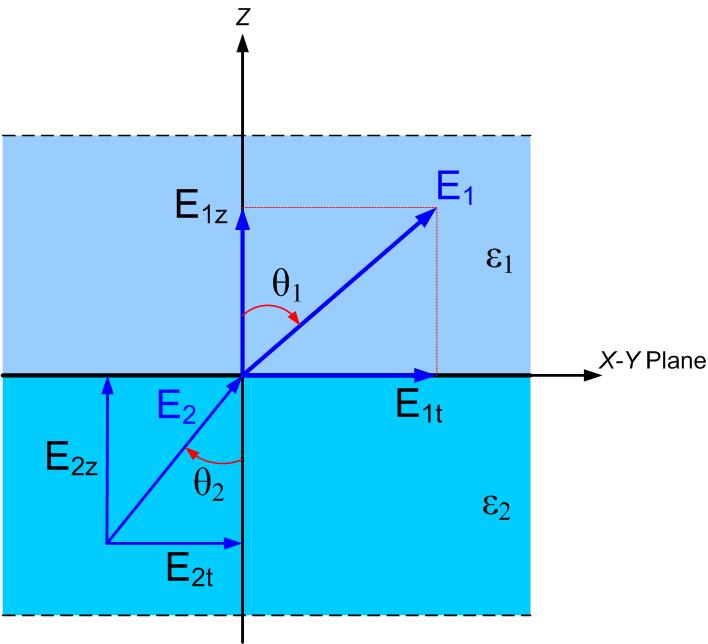
\includegraphics[scale=0.4]{../jpg/boundaryconditions.jpg}
\end{center}
\caption{Boundary Conditions for Electric Field.}
\label{fig:BoundaryCondition}
\end{figure}


%\begin{figure}[htbp]
%\centering
%\begin{tabular}{cc}

%    % Requires \usepackage{graphicx}

%   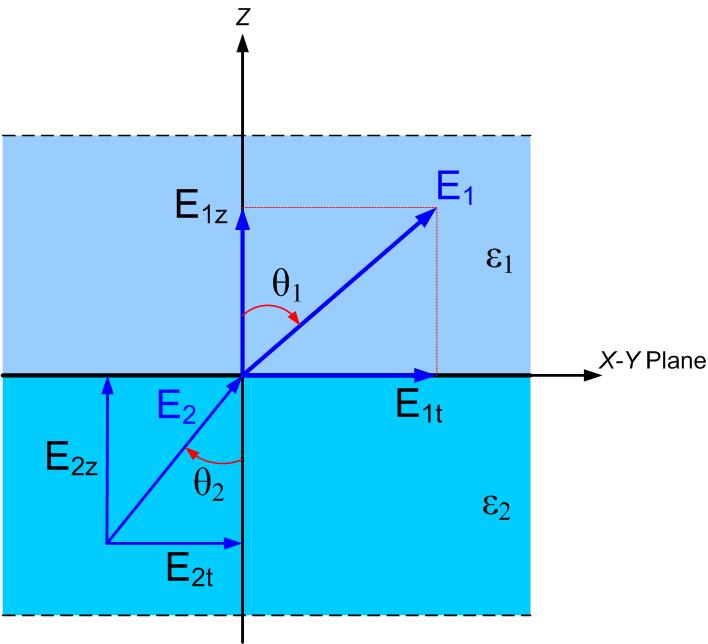
\includegraphics[width=60mm]{../jpg/boundaryconditions.jpg} &

%    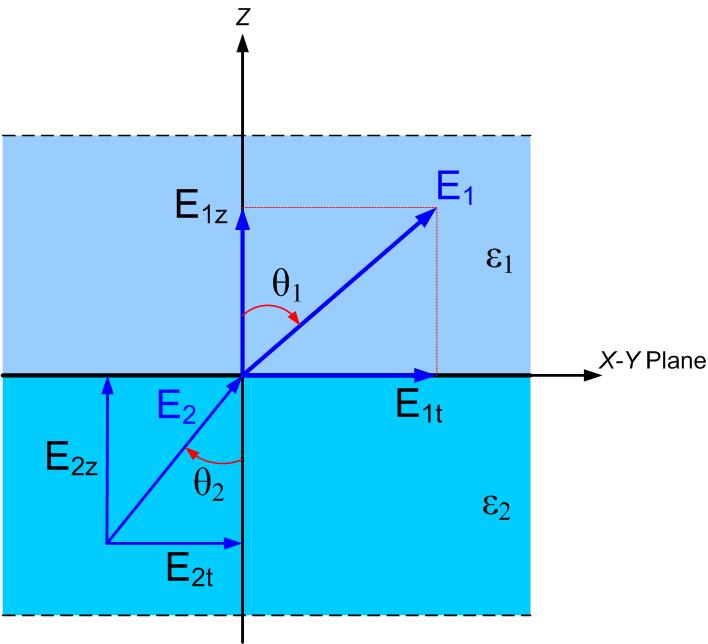
\includegraphics[width=60mm]{../jpg/boundaryconditions.jpg}\\

%    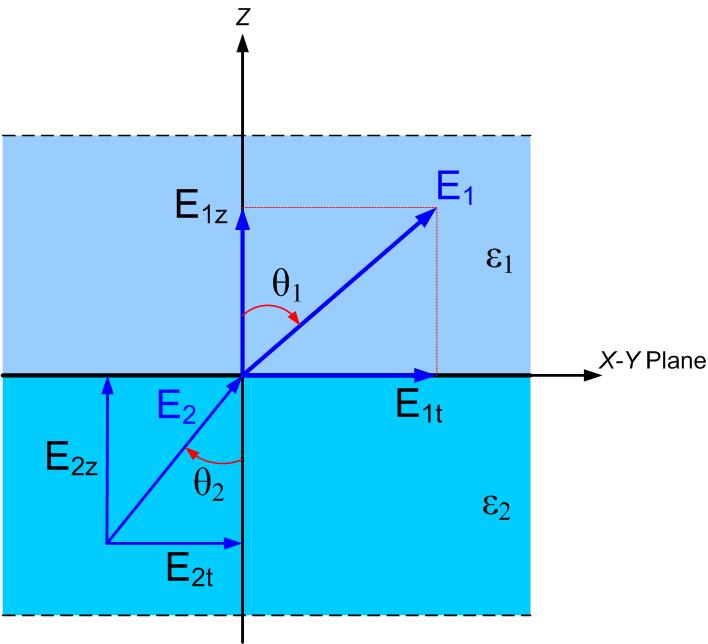
\includegraphics[width=60mm]{../jpg/boundaryconditions.jpg}&

%    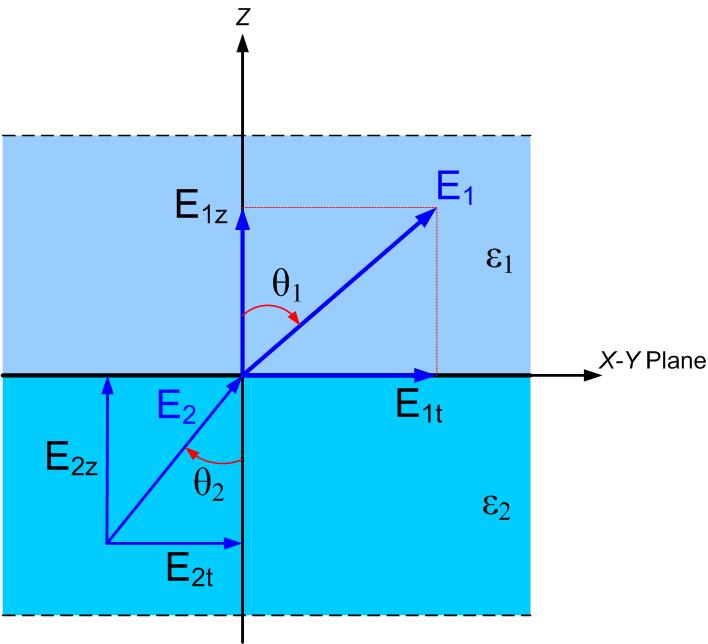
\includegraphics[width=60mm]{../jpg/boundaryconditions.jpg}

%  \end{tabular}
%\end{figure}


   \begin{question}
 The four equations below show the tangential and normal electric field at the boundary of two dielectrics. Dielectric 1 is a Teflon with a relative dielectric constant of 2.2, and dielectric 2 is Silicon with a relative dielectric constant of 11.2. Which equation represents a possible electric field? 
   \begin{multipleChoice}
     \choice{$2.2 \,E_{1t}= 11.2 \,E_{2t}$ and $E_{1n}=  E_{2n}$}
     \choice[correct]{$E_{1t}=E_{2t}$ and $2.2 \,E_{1n}= 11.2 \,E_{2n}$ }
     \choice{$2.2 \,E_{1t}= 11.2 \,E_{2t}$ and $ E_{1n}= E_{2n}$}
     \choice{$E_{1t}=E_{2t}$ and $11.2 \, E_{1n}= 2.2 \, E_{2n}$}
   \end{multipleChoice}
   \end{question}
   

\section{Boundary conditions at a conductor-dielectric boundary}

The electric field inside perfect conductors $\sigma \rightarrow \infty$ is zero. Ohm's law states that 

\begin{equation}
E=\frac{J}{\sigma}
\end{equation}


When $\sigma \rightarrow \infty$, from the above equation, we see that the electric field is zero. This means that at the boundary of the dielectric and metal, the tangential field in the dielectric must be zero as well, and the only field at the boundary of a metal is the normal electric field $D_n$, and it is equal to the induced charge at the surface of the conductor.

\begin{equation}
D_n = \rho_s
\end{equation}

Figure \ref{fig:BoundaryConditionMetal} shows the field at the boundary of the metallic sphere. 




\begin{figure}[htbp]
\begin{center}
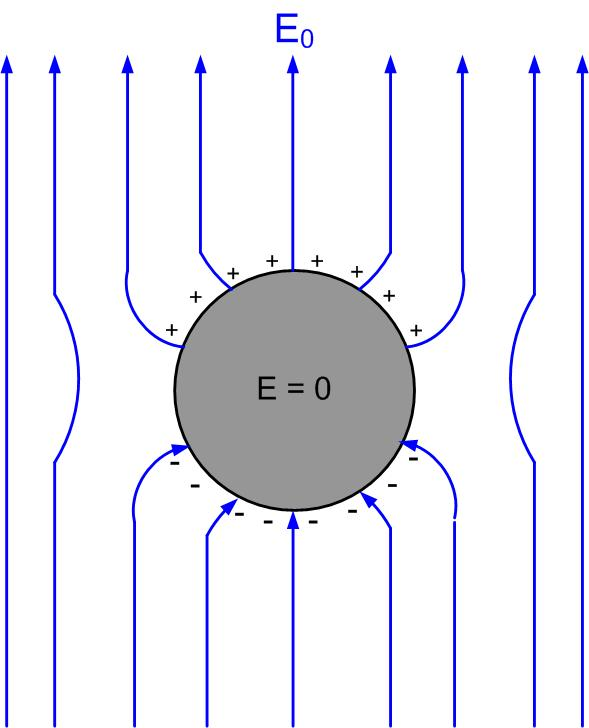
\includegraphics[scale=0.5]{../jpg/metalsphereinefield.jpg}
\end{center}
\caption{Metallic sphere in an external electric field.}
\label{fig:BoundaryConditionMetal}
\end{figure}


\section{Proof of boundary conditions}

We will now use Maxwell's equations to derive the electrostatic boundary conditions. 

First, we will use Gauss's law to find the normal component of the fields at the boundary between two dielectrics, as shown in Figure \ref{fig:BoundaryConditionNormal}. As we can see from the figure, the flux of the electric field exists through both bases and the side of the cylinder. We can find the components of the fields in both dielectrics, one parallel to the boundary x and one perpendicular to the boundary, in the direction of y.

\begin{eqnarray}
\vec{E_1}= \vec{E_{1x}}+\vec{E_{1y}}= E_{1x} \vec{x}+E_{1y} \vec{y} \\
\vec{E_2}= \vec{E_{2x}}+\vec{E_{2y}}= E_{2x} \vec{x}+E_{2y} \vec{y}
\end{eqnarray}


The tangential components of the fields produce flux through the sides, and normal components produce flux through the bases.  Since we are interested in what happens at the boundary, we will let the height of the cylinder be infinitesimally small $h \rightarrow 0$. Because the height of the cylinder is zero, and therefore the surface area is zero, the flux through the side surface S3 is zero. The flux through the top and bottom surfaces will only exist due to the normal components of the field.

\begin{eqnarray}
\oint_S \vec{D} \cdot \vec{dS} = Q_{inS} \\
\int_{S1} \vec{D} \cdot \vec{dS}  +\int_{S2} \vec{D} \cdot \vec{dS}+\int_{S3} \vec{D} \cdot \vec{dS}  =  Q_{inS} \\
\int_{S1} \vec{D} \cdot \vec{dS}  +\int_{S2} \vec{D} \cdot \vec{dS} +0 = Q_{inS} \\
\int_{S1} (\epsilon_1 E_{1n}\vec{y}+\epsilon_1 E_{1t}\vec{x}) \cdot dS\vec{y}  +(\epsilon_2 E_{2n}\vec{y}+\epsilon_2 E_{2t}\vec{x}) \cdot dS\vec{y} = Q_{inS}\\
-\epsilon_{1} E_{1n} S + \epsilon_2 E_{2n} S = Q_{inS}  \\
\epsilon_2 E_{2n} -\epsilon_{1} E_{1n}= \frac{Q_{inS}}{S} 
\end{eqnarray}




\begin{figure}[htbp]
\begin{center}
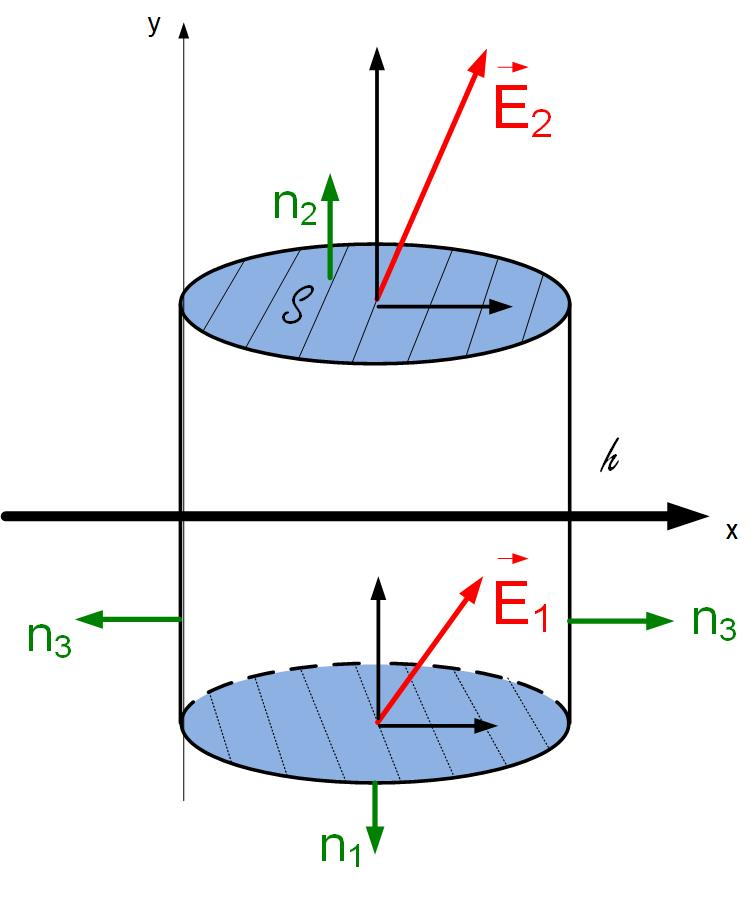
\includegraphics[scale=0.5]{../jpg/BoundaryConditionsNormal.jpg}
\end{center}
\caption{Derivation of equation for normal components of electric field on the boundary of two dielectrics.}
\label{fig:BoundaryConditionNormal}
\end{figure}


The tangential components of the field can be obtained from the equation for Faraday's law for static fields, as shown in Figure \ref{fig:BoundaryConditionTangential}. We choose a rectangular contour, as shown in the figure with length l and width w. Since again we are interested in the boundary, we will let the width of the contour go to zero. The integral along the w-pieces will then be zero. The integral along the l-pieces of contour will depend on the orientation of contour, and we will pick a counter-clockwise path. Because of the counter-clockwise path, the x-component of the $E_1$ field will be negative, and we have that the x-components of the fields in two dielectrics have to be the same.

\begin{eqnarray}
\oint_C \vec{E} \cdot \vec{dl}=0 \\
\int_{l1} (E_{1x} \vec{x}+E_{1y} \vec{y}) \cdot dy \vec{y} +\int_{l2} (E_{2x} \vec{x}+E_{2y} \vec{y}) \cdot dy \vec{y} =0 \\
-E_{1x} l + E_{2x} l = 0 \\
E_{1x}  = E_{2x}
\end{eqnarray}


\begin{figure}[htbp]
\begin{center}
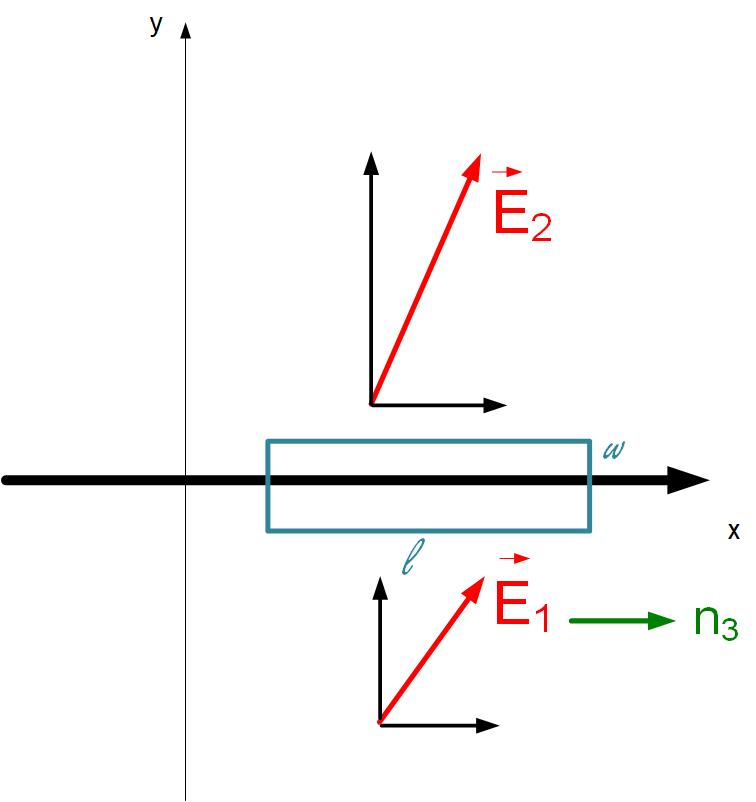
\includegraphics[scale=0.5]{../jpg/BoundaryConditionsTang.jpg}
\end{center}
\caption{Derivation of equation for tangential components of electric field on the boundary of two dielectrics.}
\label{fig:BoundaryConditionTangential}
\end{figure}



















\end{document} 

